\documentclass[tikz]{standalone}
\usepackage{amsmath,mathtools}
\begin{document}
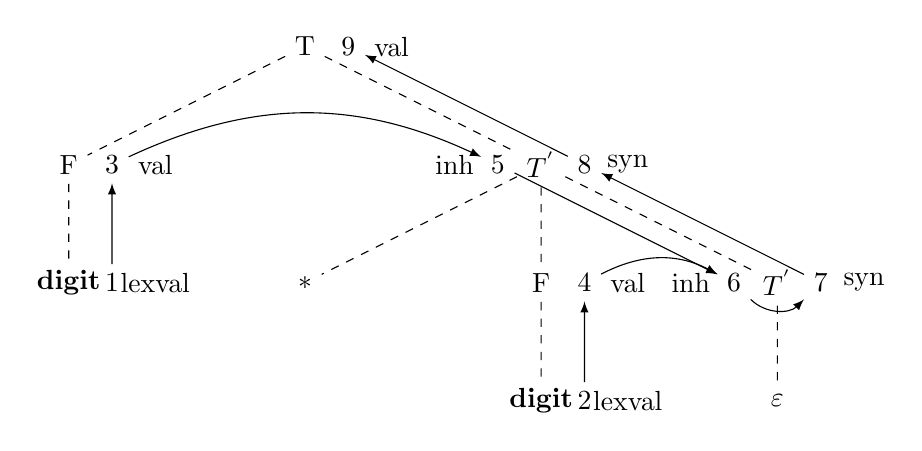
\begin{tikzpicture}[
  level/.style={sibling distance=6cm/#1},
  emph/.style={edge from parent/.style={dashed,draw}},
  norm/.style={edge from parent/.style={solid,draw}}
  ]
  \node (NRoot) {T}
  child[emph] {
    node (N1L) {F}
    child {
      node (N1L2) {\bf digit}
    }
  }
  child[emph] {
    node (N1R) {\(T^{'}\)}
    child {
      node (N1R2L) {\(*\)}
    }
    child {
      node (N1R2M) {F}
      child {
        node (N1R2M3) {\bf digit}
      }
    }
    child {
      node (N1R2R) {\(T^{'}\)}
      child {
        node (N1R2R3) {\(\varepsilon\)}
      }
    }
  };

  \path (N1L2) ++(0.55,0) node (N1L2syn) {1} -- ++(0.55,0) node {lexval};
  \path (N1L) ++(0.55,0) node (N1Lsyn) {3} -- ++(0.55,0) node {val};
  \path (N1R) ++(-0.55,0) node (N1Rinh) {5} -- ++(-0.55,0) node {inh};
  \path (N1R) ++(0.55,0) node (N1Rsyn) {8} -- ++(0.55,0) node {syn};
  \path (N1R2M) ++(0.55,0) node (N1R2Msyn) {4} -- ++(0.55,0) node {val};
  \path (N1R2M3) ++(0.55,0) node (N1R2M3syn) {2} -- ++(0.55,0) node {lexval};
  \path (N1R2R) ++(-0.55,0) node (N1R2Rinh) {6} -- ++(-0.55,0) node {inh};
  \path (N1R2R) ++(0.55,0) node (N1R2Rsyn) {7} -- ++(0.55,0) node {syn};
  \path (NRoot) ++(0.55,0) node (NRootsyn) {9} -- ++(0.55,0) node {val};

  \path[-latex,black,draw]
  (N1L2syn)   edge                    (N1Lsyn)
  (N1Lsyn)    edge[out=25,in=155]     (N1Rinh)
  (N1Rinh)    edge                    (N1R2Rinh)
  (N1R2M3syn) edge                    (N1R2Msyn)
  (N1R2Msyn)  edge[out=27.5,in=152.5] (N1R2Rinh)
  (N1R2Rinh)  edge[out=315,in=225]    (N1R2Rsyn)
  (N1R2Rsyn)  edge                    (N1Rsyn)
  (N1Rsyn)    edge                    (NRootsyn)
  ;
\end{tikzpicture}
\end{document}
